\subsection{Struttura del \textit{database}}
La prima attività chiamata "Studio degli applicativi e del \textit{database}", come introdotto nel capitolo \ref{chap:vincoli temporali}, 
vede come obiettivo lo studio delle tecnologie, del codice e del \textit{database} utilizzato dall'applicazione. Ho cominciato quindi 
dallo studio dall'architettura del \textit{database}.\\

\begin{figure}[H]
    \centering
    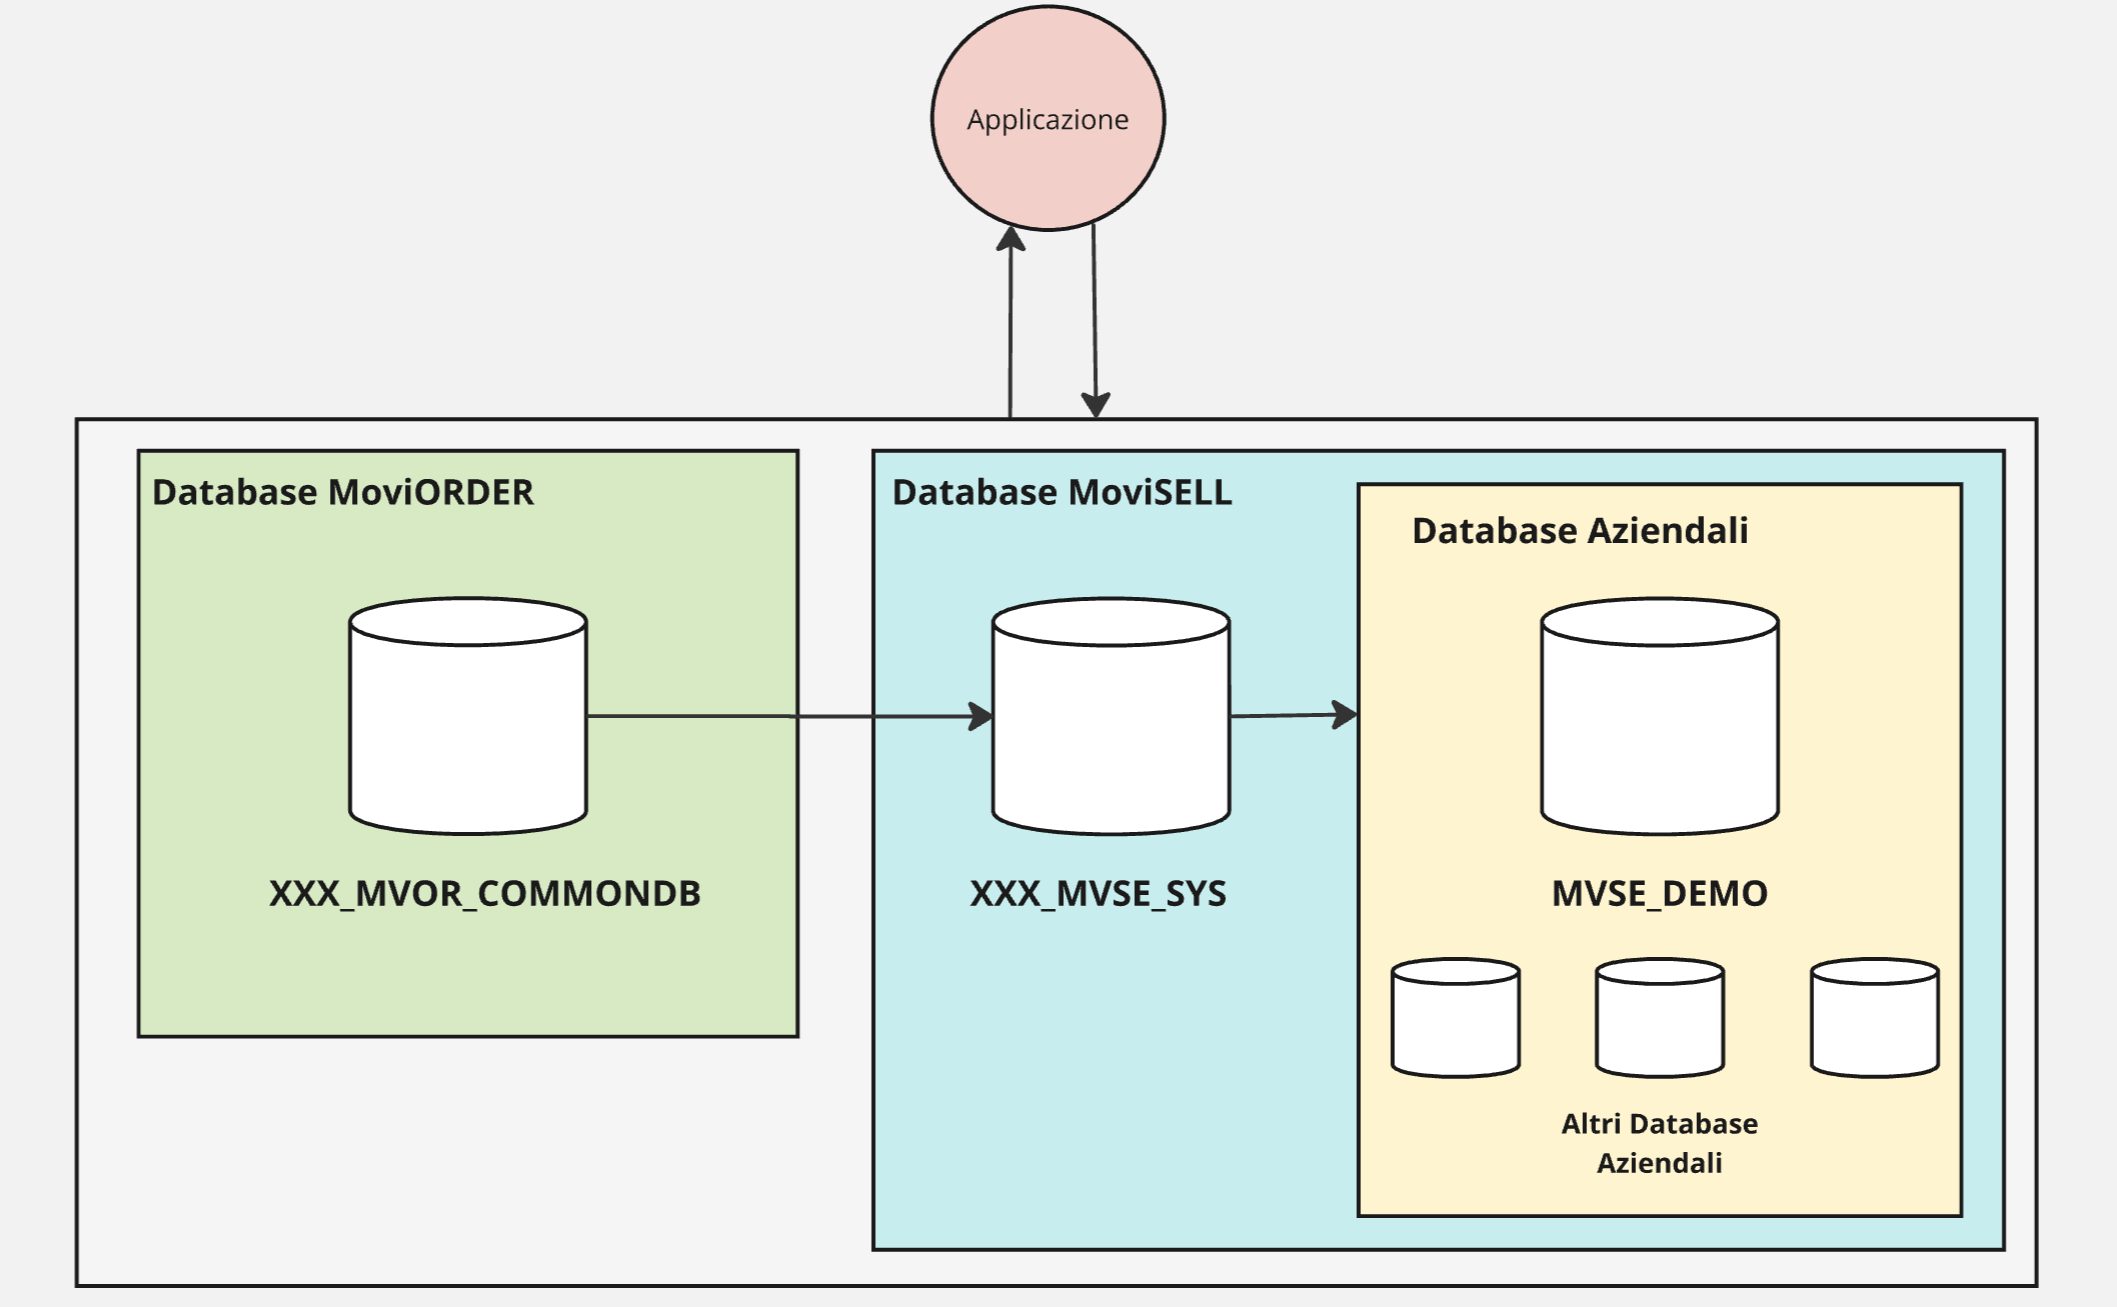
\includegraphics[alt={\textit{Database} di MoviORDER}, width=0.7\textwidth]{img/database.png}
    \caption {\textit{Database} di MoviORDER.}
    \label{fig:database}
\end{figure}

Come illustrato nella figura \ref{fig:database}, l'infrastruttura dati dell'applicazione {\movi} si articola su tre 
\textit{database} distinti: \texttt{XXX\_MVOR\_COMMONDB}, e i \textit{database} condivisi con l'applicazione 
MoviSELL, ovvero \texttt{XXX\_MVSE\_SYS} e \texttt{MVSE\_DEMO}.\\
\texttt{XXX\_MVOR\_COMMONDB} (che per brevità chiameremo \textit{common database}), contiene i dati relativi a gli utenti di MoviORDER. 
Esso conserva informazioni necessarie all'applicazione come: credenziali di accesso, stato di validità della licenza, 
configurazioni dell'interfaccia utente, dettagli del dispositivo, indirizzi email e altri parametri necessari al corretto 
funzionamento del \textit{software}. Questi dati sono fondamentali per i processi di autenticazione e inizializzazione 
dell'applicazione.\\
Ogni azienda ha il proprio \textit{database} dedicato, che chiameremo \textit{company}, in cui vengono conservati tutti i dati 
a lei inerenti come: anagrafica clienti, catalogo prodotti, politiche di sconto personalizzate, profili degli agenti 
aziendali ecc. Per ogni \textit{company database} viene assegnato un nome del tipo MVSE\_[nome azienda], nel mio caso per lavorare 
in locale mi è stato fornito un \textit{database} di prova chiamato \texttt{MVSE\_DEMO}.\\
Quindi abbiamo \texttt{XXX\_MVSE\_SYS}, il cui scopo è quello di fare da \textit{router}, infatti il \textit{common database} contiene 
un campo nella tabella \texttt{User} chiamato \texttt{CompanyCode} che agisce da chiave esterna assegnando ad ogni utente di {\movi} 
un \textit{company database } di riferimento. Questo \texttt{CompanyCode} viene utilizzato dalle \gls{api} come chiave per il 
\textit{router database} per ottenere la stringa di connessione al \textit{company database} durante la fase di autenticazione dell'
utente.\\
Questa architettura garantisce una gestione efficiente e scalabile dei dati, consentendo una separazione netta tra informazioni 
riguardanti l'applicazione e i dati specifici delle aziende, oltre a fornire un meccanismo flessibile per l'indirizzamento 
delle connessioni ai \textit{database} aziendali.